\section{Задание 4. Поверхности второго порядка}

\textbf{Условие.}

Даны $T_1$ и $T_2$ – тела, ограниченные поверхностями не выше второго порядка.
Тело $T_1$ изображено своим сечением в плоскости $Oyz$. Проекцией тела на плоскость $Oxz$ является круг.
Тело $T_2$ задано уравнениями ограничивающих поверхностей.

\begin{enumerate}
    \item Запишите уравнения и названия поверхностей, ограничивающих тело $T_1$.
    \item Изобразите тело $T_2$ и его проекции на координатные плоскости.
\end{enumerate}
\vspace{3mm}

\begin{multicols}{2}
    \begin{center}
    Тело $T_1$: \vspace{2mm}

    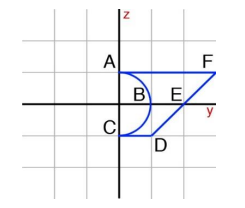
\includegraphics{images/4a1}

    Тело $T_2$: \vspace{2mm}

    \begin{cases}
        y + \sqrt{1 - x^2 - z^2} = 0,\\
        y + 2\sqrt{x^2 + z^2} = 2
    \end{cases}\\
    \end{center}
\end{multicols}
\vspace{10mm}
\textbf{Решение.}

It is empty but you can fill it!

\textit{Ответ}:  It is empty but you can fill it!
\clearpage
